%%%%%%%%%%%%%%%%%%%%%%%%%%%%%%%%%%%%%%%%%%%%%%%%%%%%%%%%%%%%%%%%%%%%%%
%
% Investigation into the architecture of epistasis
%
%%%%%%%%%%%%%%%%%%%%%%%%%%%%%%%%%%%%%%%%%%%%%%%%%%%%%%%%%%%%%%%%%%%%%%
%
%%% Preamble

\documentclass[paper=a4, fontsize=11pt]{scrartcl}         % Article class of KOMA-script with 11pt font and a4 format
\usepackage[T1]{fontenc}
\usepackage{fourier}
\usepackage{float}
\usepackage{placeins}
\usepackage[english]{babel}                     % English language/hyphenation
\usepackage[protrusion=true,expansion=true]{microtype}        % Better typography
\usepackage{amsmath,amsfonts,amsthm}                % Math packages
\usepackage[pdftex]{graphicx}                   % Enable pdflatex
\usepackage{url}
\usepackage{multicol}
\usepackage{lscape}
\usepackage{parskip}



%%% Custom sectioning (sectsty package)
\usepackage{sectsty}                        % Custom sectioning (see below)
\allsectionsfont{\centering \normalfont\scshape}          % Change font of al section commands

%%% Custom headers/footers (fancyhdr package)
\usepackage{fancyhdr}
\pagestyle{fancyplain}
\fancyhead{}                            % No page header
\fancyfoot[L]{}                           % Empty 
\fancyfoot[C]{}                           % Empty
\fancyfoot[R]{\thepage}                       % Pagenumbering
\renewcommand{\headrulewidth}{0pt}                  % Remove header underlines
\renewcommand{\footrulewidth}{0pt}                  % Remove footer underlines
\setlength{\headheight}{13.6pt}
\setlength{\parindent}{0pt}

\usepackage{tabularx,ragged2e,booktabs,caption}
\newcolumntype{C}[1]{>{\Centering}m{#1}}
\renewcommand\tabularxcolumn[1]{C{#1}}

%%% Equation and float numbering
\numberwithin{equation}{section}                  % Equationnumbering: section.eq#
\numberwithin{figure}{section}                    % Figurenumbering: section.fig#
\numberwithin{table}{section}                   % Tablenumbering: section.tab#

%%% Referencing
\bibliographystyle{naturemag}

%%% Figures
\graphicspath{{/Users/jpowell/repo/eQTL-2D/investigation/docs/figures/}}

%%% Maketitle metadata
\newcommand{\horrule}[1]{\rule{\linewidth}{#1}}           % Horizontal rule

\title{
    %\vspace{-1in}  
    \usefont{OT1}{bch}{b}{n}
    \normalfont \normalsize \textsc{University of Queensland} \\ [25pt]
    \horrule{0.5pt} \\[0.4cm]
    \huge Epistasis follow-up \\[0.3cm]
        \huge *** summary *** \\
    \horrule{2pt} \\[0.5cm]
    \date{}
}

\begin{document}

%%%%%%%%%%%%%%%%%%%%%%%%%%%%%%%%%%%%%%%%%%%%%%%%%%%%%%%%%%%%%%%%%%%%%%%%%%%%%%%%%%%%%
%%%%%%%%%%%%%%%%%%%%%%%%%%%%%%%%%%%%%%%%%%%%%%%%%%%%%%%%%%%%%%%%%%%%%%%%%%%%%%%%%%%%%
%%%%%%%%%%%%%%%%%%%%%%%%%%%%%%%%%%%%%%%%%%%%%%%%%%%%%%%%%%%%%%%%%%%%%%%%%%%%%%%%%%%%%


%%% Begin document
\maketitle


%%%%%%%%%%%%%%%%%%%%%%%%%%%%%%%%%%%%%%%%%%%%%%%%%%%%%%%%%%%%%%%%%%%%%%%%%%%%%%%%%%%%%
%%%%%%%%%%%%%%%%%%%%%%%%%%%%%%%%%%%%%%%%%%%%%%%%%%%%%%%%%%%%%%%%%%%%%%%%%%%%%%%%%%%%%
%%%%%%%%%%%%%%%%%%%%%%%%%%%%%%%%%%%%%%%%%%%%%%%%%%%%%%%%%%%%%%%%%%%%%%%%%%%%%%%%%%%%%

\newpage
\section*{Original analysis summary}
\noindent


Original discovery analysis identified 501 interactions comprising of 781 unique SNPs and 238 genes (probes). These were 26 cis-cis, 462 cis-trans and 13 trans trans. The majority of our discovery interactions were composed of one SNP that was significantly associated with the gene expression level in the discovery data set, and one SNP that had no previous association (439 out of 501, Methods). Only nine interactions were between SNPs that both had known main effects, whereas 64 were between SNPs that had no known main effects. \\

In the original analysis the following thresholds were used; \\

\subsubsection*{Stage 1}
 
The complete exhaustive scan for 7339 probes comprises $1.03 \times 10^{15}$ $F$-tests. We used permutation analysis to estimate an appropriate significance threshold for the study. To do this we performed a further 1600 exhaustive 2D scans on permuted phenotypes to generate a null distribution of the extreme $p$-values expected to be obtained from this number of multiple tests given the correlation structure between the SNPs. We took the most extreme $p$-value from each of the 1600 scans and set the 5\% FWER to be the 95\% most extreme of these $p$-values, $T_{*} = 2.13 \times 10^{-12}$. The effective number of tests in one 2D scan being performed is therefore $N_{*} = 0.05 / T_{*} \approx 2.33 \times 10^{10}$. To correct for the testing of multiple probes we established an experiment wide threshold of $T_{e} = 0.05 / (N_{*} \times 7339) = 2.91 \times 10^{-16}$. 



\paragraph{Filtering} We used two approaches to filter SNPs from stage 1 to be tested for significant interaction effects in stage 2.

\paragraph{Filter 1} After keeping SNP pairs that surpassed the $2.91 \times 10^{-16}$ threshold in stage 1 only SNP pairs with at least 5 data points in all 9 genotype classes were kept. We then calculated the LD between interacting SNPs (amongst unrelated individuals within the discovery sample and also from 1000 genomes data) and removed any pairs with $r^2 > 0.1$ or $D'^{2} > 0.1$ to avoid the inclusion of haplotype effects and to increase the accuracy of genetic variance decomposition. If multiple SNP pairs were present on the same chromosomes for a particular expression trait then only the sentinel SNP pair was retained, \emph{i.e.} if a probe had multiple SNP pairs that were on chromosomes one and two then only the SNP pair with the most significant $p$-value was retained. At this stage 6404 filtered SNP pairs remained. 

\paragraph{Filter 2} We also performed a second filtering screen applied to the list of SNP pairs from stage 1 that was identical to filter 1 but an additional step was included where any SNPs that had previously been shown to have a significant additive or dominant effect ($p < 1.29 \times 10^{-11}$) were removed, creating a second set of 4751 unique filtered SNP pairs.

\subsubsection*{Stage 2}

To ensure that interacting SNPs were driven by epistasis and not marginal effects we performed a nested ANOVA on each pair in the filtered set to test if the interaction terms were significant. We did this by contrasting the full genetic model (8 \emph{d.f.}) against the reduced marginal effects model which included the additive and dominance terms at both SNPs (4 \emph{d.f.}). Thus, a 4 \emph{d.f.} $F$-test was performed on the residual genetic variation, representing the contribution of epistatic variance. Significance of epistasis was determined using a Bonferroni threshold of $0.05 / (6404+4751) = 4.48 \times 10^{-6}$. This resulted in 406 and 95 SNP pairs with significant interaction terms from filters 1 and 2, respectively.


\subsection*{Type 1 error rate}

Using a Bonferroni correction of $0.05$ in the second stage of the two stage discovery scan implies a type 1 error rate of $\alpha = 0.05$. However, this could be underestimated because the number tests performed in the second stage depends on the number of tests in the first stage, and this depends on statistical power and model choice. We performed simulations to estimate the type 1 error rate of this study design.

We assumed a null model where there was one true additive effect and 7 other terms with no effect. To simulate a test statistic we simulated 8 z-scores, $z_1 \sim N(\sqrt{NCP}, 1)$ and $z_{2..8} \sim N(0,1)$. Thus $z_{full} = \sum^8_{i=1}{z_i} \sim \chi^{2}_{8}$ (representing the 8 d.f. test) and $z_{int} = \sum^8_{i=5}{z_i} \sim \chi^{2}_{4}$ (representing the 4 d.f. test where the null hypothesis of no epistasis is true). For a particular value of $NCP$ we simulated 100,000 $z$ values, and calculated the $p_{full}$-value for the $z_{full}$ test statistic. The $n_{int}$ test statistics with $p_{full} < 2.31 \times 10^{-16}$ were kept for the second stage, where the type 1 error rate of stage 2 was calculated as the proportion of $p_{int} < 0.05 / n_{int}$. The power at stage 1 was calculated as $n_{int} / 100,000$. This procedure was performed for a range of $NCP$ parameters that represented power ranging from $\sim 0$ to $\sim 1$.

\newpage

\section*{Methods and results}

The following analyses have been conducted; \\

\textbf{1. GWAS based determination of the empirical p-values for each of the 501 interactions} \\

The initial analysis used F-tests and some simulation work to determine the expected Type 1 error rate in the 1st stage of the discovery process. The 1st stage was followed by a 2nd stage where the interaction model was fitted. Subsequent simulations and theoretical calculations have suggested that the Type 1 error rate of the 2nd stage is not correct when there is a large main effect and / or in the presence of LD.  \\

a. The SNP with largest additive effect was identified for each pair of the 501 original epistasis SNPs. \\

b. The largest additive SNP was treated as a fixed SNP and a genome-wide analysis using the 8df and 4df epistasis model was performed. \\

c. This generated $\approx 500,000$ interaction p-values. The sample snp-pair filtering as used in the manuscript was applied. Namely, LD ($r^2$ < 0.1), nclass $=$ 9, and minclass $>$ 5. Any SNP with +/- 5MB of original epistasis SNP pairs were also removed. \\

d.  The filtered interaction p-values were used to determine the empirical distribution of null p-values. \\

e. Summary information such as median lambda were calculated from the filtered interaction p-values. \\

\textbf{2. Permutation based determination of the empirical p-values for each of the 501 interactions} \\

a. As before, the SNP with largest additive effect was identified for each pair of the 501 original epistasis SNPs. \\

b. Genotypes at the corresponding epistatitic ''co-SNP'' were randomly shuffled (no replacement) amongst individuals. \\

c. Interaction p-values and text statistics were calculated using the same methods. \\

d. For each pair (\emph{n}=501) this analysis was performed 10,000,000 times. \\

e. The same filtering was applied (although $r^2$ not required). \\

f. The empirical \emph{p}-value determined based on rank of observed \emph{F}-Statistic 

\newpage

\begin{landscape}

\begin{table}[ht]
\centering
\begin{tabular}{rrrrrr}
  \hline
 & F & P & nclass & minclass & LD \\ 
  \hline
1 & 0.36 & 0.78 & 8.00 & 1.00 & 0.00 \\ 
  2 & 0.44 & 0.72 & 8.00 & 7.00 & 0.00 \\ 
  3 & 0.33 & 0.85 & 9.00 & 2.00 & 0.00 \\ 
  4 & 0.36 & 0.84 & 9.00 & 6.00 & 0.01 \\ 
  5 & 0.29 & 0.75 & 6.00 & 1.00 & 0.00 \\ 
  6 & 0.12 & 0.89 & 6.00 & 1.00 & 0.00 \\
  ... & ... & ... & ... & ...& ... \\ 
   \hline
\end{tabular}
\caption*{Header of output for a single pair}
\end{table}

\vspace{2cm}


\begin{table}[ht]
\centering
\tiny
\begin{tabular}{llllllllrrrlllllll}
  \hline
 probename & snp1 & snp2 & nclass9 & minclass5 & LD01 & npass & nsnps & filter & p\_egcut & p\_fehr & $\lambda$ & nthres & Fe & N\_Fe & F\_emp & P\_emp & type1 \\ 
  \hline
ILMN\_1651385 & rs7989895 & rs4846085 & 419387 & 285750 & 506818 & 269121 & 506818 & 1.00 & 0.25 & 0.61 & 1.61 & 4 & 9.43 & 0 & 8.95 & 6.35 & 0.10 \\ 
ILMN\_1651705 & rs872311 & rs11032695 & 419021 & 278721 & 511121 & 260851 & 511121 & 1.00 & 0.30 & 0.26 & 1.12 & 1 & 9.41 & 0 & 7.75 & 5.41 & 0.05 \\ 
ILMN\_1651886 & rs7108734 & rs12784396 & 427787 & 319167 & 501291 & 305496 & 501291 & 1.00 & 0.01 & 0.21 & 1.07 & 0 & 9.5 & 0 & 7.4 & 5.13 & 0.05 \\ 
ILMN\_1652333 & rs898095 & rs9892064 & 442554 & 336649 & 515007 & 322786 & 515007 & 2.00 & 29.39 & 28.24 & 1.34 & 7 & 9.53 & 0 & 9.48 & 6.77 & 0.07 \\ 
ILMN\_1653205 & rs12429804 & rs2896452 & 383323 & 213815 & 507099 & 183628 & 507099 & 1.00 & 0.02 & 0.29 & 1.78 & 24 & 9.22 & 4 & 10.56 & 7.63 & 0.11 \\ 
ILMN\_1653205 & rs12454561 & rs2896452 & 386460 & 215536 & 511390 & 185098 & 511390 & 1.00 &  & 0.31 & 1.78 & 25 & 9.22 & 4 & 10.56 & 7.63 & 0.11 \\ 
ILMN\_1653205 & rs2896452 & rs1004564 & 373839 & 208706 & 494954 & 179170 & 494954 & 1.00 & 0.18 & 0.38 & 1.78 & 23 & 9.2 & 2 & 10.08 & 7.25 & 0.11 \\ 
ILMN\_1653205 & rs7152284 & rs2896452 & 385471 & 215221 & 509793 & 184859 & 509793 & 1.00 & 0.07 & 2.18 & 1.78 & 23 & 9.22 & 3 & 10.56 & 7.63 & 0.11 \\ 
ILMN\_1653205 & rs8051751 & rs2896452 & 386341 & 215644 & 511501 & 185188 & 511501 & 1.00 & 0.18 & 1.39 & 1.78 & 24 & 9.22 & 4 & 10.56 & 7.63 & 0.11 \\ 
ILMN\_1654545 & rs4333645 & rs1455268 & 421112 & 307876 & 495374 & 294544 & 495374 & 2.00 & 0.01 & 0.10 & 1.45 & 4 & 9.48 & 0 & 9.14 & 6.5 & 0.08 \\ 
ILMN\_1656378 & rs10906857 & rs12490878 & 418379 & 314668 & 489831 & 301252 & 489831 & 1.00 & 0.34 & 0.42 & 1.1 & 1 & 9.49 & 0 & 7.69 & 5.36 & 0.05 \\ 
ILMN\_1658247 & rs11613438 & rs1047944 & 402228 & 251785 & 490871 & 234981 & 490871 & 2.00 & 1.55 & 1.27 & 1.53 & 21 & 9.35 & 1 & 9.73 & 6.97 & 0.09 \\ 
   \hline
\end{tabular}
\caption*{Header of summary output for 501 pairs}
\end{table}


\end{landscape}

%%%%%%%%%%%%%%%%%%%%%%%%%%%%%%%%%%%%%%%%%%%%%%%%%%%%%%%%%%%%%%%%%%
%%%%%%%%%%%%%%%%%%%%%%%%%%%%%%%%%%%%%%%%%%%%%%%%%%%%%%%%%%%%%%%%%%
%%%%%%%%%%%%%%%%%%%%%%%%%%%%%%%%%%%%%%%%%%%%%%%%%%%%%%%%%%%%%%%%%%


\newpage
\begin{figure}[H]
\centering
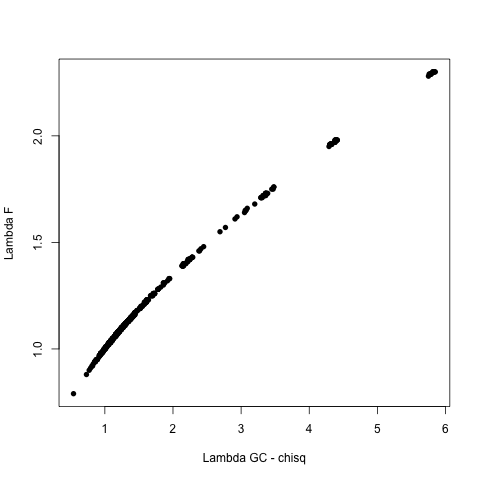
\includegraphics[width=4in]{lambda.png}
\caption*{Figure | Distribution of median lambda from the 501 fixed SNP analysis. Red denotes original pairs identified from filter 2 - i.e. no previous study-wide additive effects. Black denotes the original filter 1 pairs}
\end{figure}

\vspace{1cm}

\begin{table}[ht]
\centering
\begin{tabular}{rlllll}
  \hline
probename & snp1 & snp2 & meanlambda & npairs \\ 
  \hline
ILMN\_1704730 & rs1884655 & rs10255470 & 2.88 & 10 \\ 
ILMN\_1710752 & rs2123758 & rs2786014 & 2.15 & 8 \\ 
ILMN\_1717234 & rs1157079 & rs7733671 & 4.31 & 17 \\ 
ILMN\_1720059 & rs12435486 & rs7837237 & 2.29 & 7 \\ 
ILMN\_1738784 & rs10930170 & rs12120009 & 2.24 & 6 \\ 
ILMN\_1755589 & rs11080134 & rs11169322 & 1.16 & 6 \\ 
ILMN\_1786426 & rs2839013 & rs8106959 & 5.65 & 20 \\ 
ILMN\_1804396 & rs1293455 & rs2655991 & 1.38 & 7 \\ 
ILMN\_2313158 & rs10869600 & rs13069559 & 3.15 & 15 \\ 
ILMN\_2372639 & rs17159840 & rs10059004 & 4.17 & 17 \\ 
ILMN\_3231952 & rs12947580 & rs8079215 & 2.16 & 6 \\ 
   \hline
\end{tabular}
\caption*{Mean lambda per probe, when 5 or more interactions are identified amongst the 501 pairs}
\end{table}

%%%%%%%%%%%%%%%%%%%%%%%%%%%%%%%%%%%%%%%%%%%%%%%%%%%%%%%%%%%%%%%%%%
%%%%%%%%%%%%%%%%%%%%%%%%%%%%%%%%%%%%%%%%%%%%%%%%%%%%%%%%%%%%%%%%%%
%%%%%%%%%%%%%%%%%%%%%%%%%%%%%%%%%%%%%%%%%%%%%%%%%%%%%%%%%%%%%%%%%%
\newpage

\begin{figure}[H]
\centering
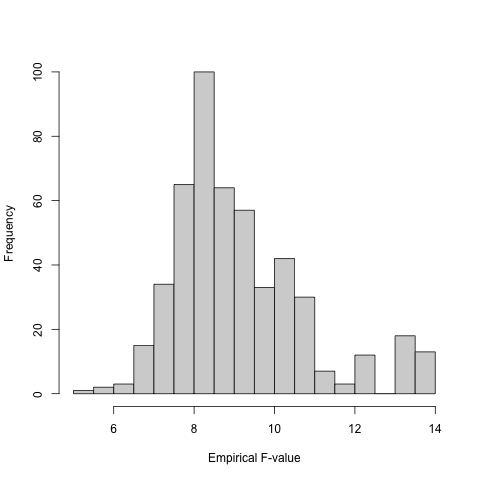
\includegraphics[height=3in]{empF.png}
\caption*{Figure | The F-statistic corresponding to $p=4.48^{-6}$ and df1=4, df2=842 from a $H_0$ table is 7.67. This figure shows the empirical (ranked) F-statistic corresponding to $n * 4.48^{-6}$. Where $n * 4.48^{-6} < 1$, the largest F-statistic taken. There are 96 pairs where the corresponding F statistic is less than 7.67}
\end{figure}


\begin{figure}[H]
\centering
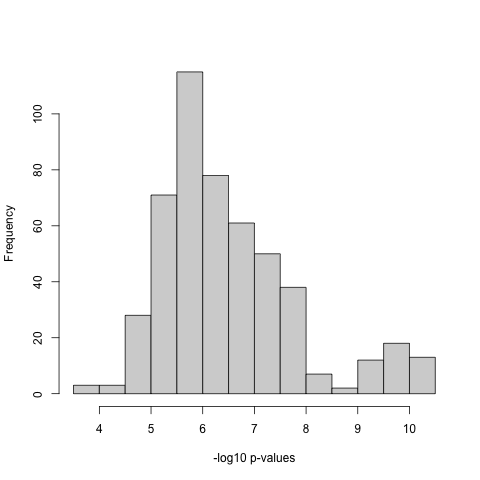
\includegraphics[height=3in]{empPval.png}
\caption*{Figure | The -log10 p-values corresponding to above F-statistics (df1=4, df2=842). The -log10 $p=4.48^{-6} = 5.35$}
\end{figure}



%%%%%%%%%%%%%%%%%%%%%%%%%%%%%%%%%%%%%%%%%%%%%%%%%%%%%%%%%%%%%%%%%%
%%%%%%%%%%%%%%%%%%%%%%%%%%%%%%%%%%%%%%%%%%%%%%%%%%%%%%%%%%%%%%%%%%
%%%%%%%%%%%%%%%%%%%%%%%%%%%%%%%%%%%%%%%%%%%%%%%%%%%%%%%%%%%%%%%%%%
\newpage

\begin{figure}[H]
\centering
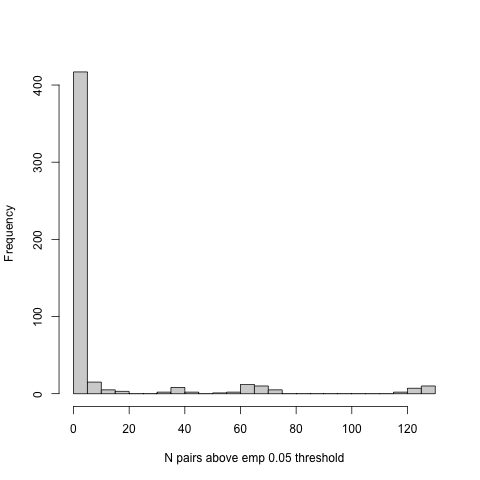
\includegraphics[height=3in]{Npairs_above_empthres.png}
\caption*{Figure | For each pair (n=501) the number of tests where the test statistic is greater than the 95th percentile of an F-dist}
\end{figure}


\begin{figure}[H]
\centering
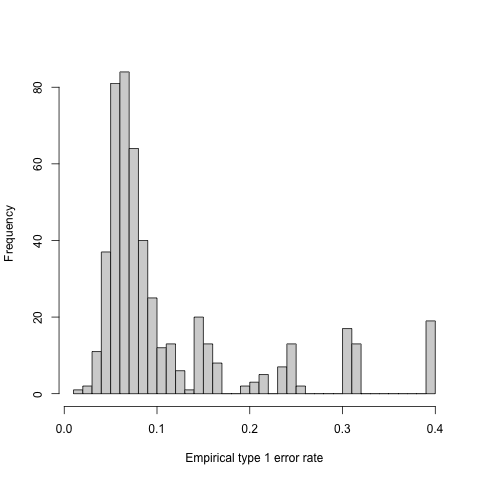
\includegraphics[height=3in]{type1.png}
\caption*{Figure | Distribution of the empirical type 1 error rate. Determined as the proportion of tests with $F > 2.38$ (95th percentile of F-dist with df1=4, df2=842)}
\end{figure}



%%%%%%%%%%%%%%%%%%%%%%%%%%%%%%%%%%%%%%%%%%%%%%%%%%%%%%%%%%%%%%%%%%
%%%%%%%%%%%%%%%%%%%%%%%%%%%%%%%%%%%%%%%%%%%%%%%%%%%%%%%%%%%%%%%%%%
%%%%%%%%%%%%%%%%%%%%%%%%%%%%%%%%%%%%%%%%%%%%%%%%%%%%%%%%%%%%%%%%%%
\newpage



\begin{table}[ht]
\centering
\begin{tabular}{llllll}
  \hline
gene & probename & snp1 & snp2 & $\lambda$ & Type1 \\ 
  \hline
ADK & ILMN\_2358626 & rs2395095 & rs10824092 & 1.15 & 0.06 \\ 
ATP13A1 & ILMN\_2134224 & rs4284750 & rs873870 & 1.82 & 0.119 \\ 
C21ORF57 & ILMN\_1795836 & rs9978658 & rs11701361 & 1.43 & 0.085 \\ 
CSTB & ILMN\_1761797 & rs9979356 & rs3761385 & 1.05 & 0.053 \\ 
CTSC & ILMN\_2242463 & rs7930237 & rs556895 & 1.12 & 0.054 \\ 
FN3KRP & ILMN\_1652333 & rs898095 & rs9892064 & 1.34 & 0.075 \\ 
GAA & ILMN\_2410783 & rs11150847 & rs12602462 & 1.38 & 0.081 \\ 
HNRPH1 & ILMN\_2101920 & rs6894268 & rs4700810 & 1.47 & 0.091 \\ 
LAX1 & ILMN\_1769782 & rs1891432 & rs10900520 & 1.22 & 0.066 \\ 
MBLN1 & ILMN\_2313158 & rs11981513 & rs13069559 & 3.36 & 0.242 \\ 
MBLN1 & ILMN\_2313158 & rs16864367 & rs13079208 & 2.28 & 0.161 \\ 
MBLN1 & ILMN\_2313158 & rs2030926 & rs13069559 & 3.39 & 0.241 \\ 
MBLN1 & ILMN\_2313158 & rs218671 & rs13069559 & 3.36 & 0.242 \\ 
MBLN1 & ILMN\_2313158 & rs2614467 & rs13069559 & 3.37 & 0.242 \\ 
MBLN1 & ILMN\_2313158 & rs7710738 & rs13069559 & 3.38 & 0.243 \\ 
MBP & ILMN\_2398939 & rs8092433 & rs4890876 & 1.19 & 0.066 \\ 
NAPRT1 & ILMN\_1710752 & rs2123758 & rs3889129 & 2.14 & 0.155 \\ 
NCL & ILMN\_2121437 & rs7563453 & rs4973397 & 1.2 & 0.065 \\ 
PRMT2 & ILMN\_1675038 & rs2839372 & rs11701058 & 2.77 & 0.199 \\ 
SNORD14A & ILMN\_1799381 & rs2634462 & rs6486334 & 2.45 & 0.168 \\ 
TMEM149 & ILMN\_1786426 & rs807491 & rs7254601 & 2.69 & 0.194 \\ 
TMEM149 & ILMN\_1786426 & rs8106959 & rs1843357 & 5.79 & 0.396 \\ 
TMEM149 & ILMN\_1786426 & rs8106959 & rs2351458 & 5.77 & 0.395 \\ 
TMEM149 & ILMN\_1786426 & rs8106959 & rs6718480 & 5.82 & 0.397 \\ 
TMEM149 & ILMN\_1786426 & rs8106959 & rs6926382 & 5.75 & 0.396 \\ 
TMEM149 & ILMN\_1786426 & rs8106959 & rs914940 & 5.76 & 0.395 \\ 
TMEM149 & ILMN\_1786426 & rs8106959 & rs9509428 & 5.82 & 0.398 \\ 
VASP & ILMN\_1743646 & rs1264226 & rs2276470 & 1.37 & 0.08 \\ 
RPL13 & ILMN\_2413278 & rs352935 & rs2965817 & 1.11 & 0.058 \\ 
TRA2A & ILMN\_1731043 & rs7776572 & rs11770192 & 1.36 & 0.079 \\ 
   \hline
\end{tabular}
\caption*{The $\lambda$ and type 1 error rates for the 30 (Bonferroni-correction) significant replicated pairs mentioned in Hemani \emph{et al}.}
\end{table}

%%%%%%%%%%%%%%%%%%%%%%%%%%%%%%%%%%%%%%%%%%%%%%%%%%%%%%%%%%%%%%%%%%
%%%%%%%%%%%%%%%%%%%%%%%%%%%%%%%%%%%%%%%%%%%%%%%%%%%%%%%%%%%%%%%%%%
%%%%%%%%%%%%%%%%%%%%%%%%%%%%%%%%%%%%%%%%%%%%%%%%%%%%%%%%%%%%%%%%%%
\newpage

2. Identify the largest additive eQTL for the probe (irrespective of effect size). Regress out the effect of the additive loci and use the adjusted phenotype for 8df and 4df model analysis. Results reported are the 8df and 4df of original pair and the empirical p-values from genome-wide analysis fitting each of the two SNPs as fixed. As before these are determined by filtering out the SNPs on the same chromosome as the original fixed SNP and also within +/- 5MB of the second SNP. \\

[Currently running]

\vspace{1cm}

2. Prediction \\

Of the 501 SNP pairs, 484 have both SNP in the EGCUT data. Most of the Inchianti SNPs need to be imputed, but we expect most to pass filtering. For pairs without and Inchianti SNP I propose using the SNP with the largest additive effect in the egcut data. \\

For each pair; \\

a. Predict the phenotype in egcut data using a predictor with effects estimated from \\

4df model (estimated in BSGS) \\
8df model (estimated in BSGS) \\
1df model (estimated in BSGS using the Inchianti snp) \\








%%%%%%%%%%%%%%%%%%%%%%%%%%%%%%%%%%%%%%%%%%%%%%%%%%%%%%%%%%%%%%%%%%%%%%%%%%%%%%%%%%%%%
%%%%%%%%%%%%%%%%%%%%%%%%%%%%%%%%%%%%%%%%%%%%%%%%%%%%%%%%%%%%%%%%%%%%%%%%%%%%%%%%%%%%%
%%%%%%%%%%%%%%%%%%%%%%%%%%%%%%%%%%%%%%%%%%%%%%%%%%%%%%%%%%%%%%%%%%%%%%%%%%%%%%%%%%%%%


%%%%%%%%%%%%%%%%%%%%%%%%%%%%%%%%%%%%%%%%%%%%%%%%%%%%%%%%%%%%%%%%%%%%%%%%%%%%%%%%%%%%%
%%%%%%%%%%%%%%%%%%%%%%%%%%%%%%%%%%%%%%%%%%%%%%%%%%%%%%%%%%%%%%%%%%%%%%%%%%%%%%%%%%%%%
%%%%%%%%%%%%%%%%%%%%%%%%%%%%%%%%%%%%%%%%%%%%%%%%%%%%%%%%%%%%%%%%%%%%%%%%%%%%%%%%%%%%%



%%%%%%%%%%%%%%%%%%%%%%%%%%%%%%%%%%%%%%%%%%%%%%%%%%%%%%%%%%%%%%%%%%%%%%%%%%%%%%%%%%%%%
%%%%%%%%%%%%%%%%%%%%%%%%%%%%%%%%%%%%%%%%%%%%%%%%%%%%%%%%%%%%%%%%%%%%%%%%%%%%%%%%%%%%%
%%%%%%%%%%%%%%%%%%%%%%%%%%%%%%%%%%%%%%%%%%%%%%%%%%%%%%%%%%%%%%%%%%%%%%%%%%%%%%%%%%%%%




%%% End document
\end{document}





